% Basic info about your document: a4 paper, 11pt font size, article style.
\documentclass[a4paper, 11pt]{article}

\usepackage{graphicx} % Enables adding figures
\usepackage[a4paper, margin=18mm]{geometry} % Let's you adjust the margins
\usepackage[T1]{fontenc} % Font helvetica
\usepackage[scaled]{helvet}
\usepackage{authblk} % multiauthor
\usepackage{multirow} % table
\usepackage[table,xcdraw]{xcolor}
\usepackage{float} % position des figures,table
\usepackage[backend=biber,style=numeric,sorting=none]{biblatex} % bibliographie

\addbibresource{bibliographie.bib} % utilise bibliographie.bib pour la bibliographie
\graphicspath{ {./figure/} } % relative path for figure
\renewcommand\familydefault{\sfdefault} % set font for all document
\renewcommand*\contentsname{Table des matières} % Rename table of contents

%Setup Titre, auteur et date
\title{
    \vspace{-2.5cm}
    \centering\includegraphics[scale=0.5]{Logos\_Hepia.png}\\
    \centering\rule{17cm}{0.1mm}\vspace*{0.4in}\\
    \centering Projet thématique MOON}
\author[1]{AYRINHAC Elisa}
\author[2]{DROUIN Clément}
\author[3]{JOUCLARD Charly}
\affil[1]{HEPIA, MT2, elisa.ayrinhac@hes-so.ch}
\affil[2]{HEPIA, MT2, clement.drouin@hes-so.ch}
\affil[3]{HEPIA, MT2, charly.jouclard@hes-so.ch}
\date{28 avril 2023}

\begin{document}

%Entete
\maketitle
\begin{center}
    \rule{\textwidth}{0.1mm}
\end{center}
%Introduction
\vspace{-1cm}
\section*{Introduction}
Le projet thématique viens se placer dans le cadre des études de bachelor en microtechnique option Bio-ingénierie.
Cette année notre cliente est une biologiste travaillant sur l'endométriose, une maladie encore peu connue touchant 1 femme sur 10.
Cette pathologie se caractérise par le développement de tissu semblable à l'endomètre hors de l'utérus.
Ces tissus peuvent proliférer dans les organes voisins comme les ovaires, l'intestins, la vessie ou même les poumons.
Les symptômes varient énormément entre les femmes mais ont retiens, le plus souvent, celui de la douleur extrême provoquer par la croissance de ces tissus.
Le but de notre projet est de créer un bio-chip qui permettrait d'étudier les tissus de l'endomètre soumis à différentes concentration d'hormones.
\newpage
%Table des matieres
\tableofcontents
\newpage
%Debut rapport
\section{Etudes préliminaire}
\subsection{Biologie}
Pour que l'expérience soit optimale, le client a besoin de suivre l'évolution d'un tissu d'endomètre sur la durée d'un cycle endométrial.
Le système doit être compact et permettre l'observation des cellules en culture ainsi que la possibilité de collecter des cellules et du milieu de culture pour analyse.
Afin mieux comprendre comment concevoir un appareil correspondant à la demande du client, une courte introduction biologique est nécessaire.
L'endomètre est un épithélium qui compose une partie de l'appareil reproducteur féminin, il tapisse les parois de la cavité utérine et est composé de 3 couches :
Le myomètre qui est la fondation de l'endomètre, la couche basale qui contient les glandes et les tissu conjonctifs et la couche fonctionnelle.
Cette dernière couche est celle qui vois sa taille changer durant le cycle menstruel qui est réglé par 4 Hormones.
L'hypothèse émise par la biologiste serais qu'il y a une influence du cycle hormonale sur l'apparition de l'endométriose.
Il y a notamment deux hormones qui sont suspecter, l'estradiol et la progestérone.
Nous allons donc devoir recrée les concentrations de ce cycle et les appliquer à des cellules in-vitro.
\subsection{Etat de l'art}
Actuellement la culture cellulaire est un procédé connu et maitriser par l'Homme qui consiste à placer des cellules dans un milieu de culture afin de les faire proliférer.
Cette méthode permet d'avoir des colonies de cellule pouvant aller jusqu'a formé des organoïdes.
Organoïdes pouvant être utilisés à des fins de recherche sur l'organe miniaturisé.
La méthode d'incubation consiste à placer dans un incubateur une colonie de cellules contenue dans un milieu nutritif.
Pour maintenir de bonnes conditions on place ces échantillons dans l'enceinte d'un incubateur qui permet d'isoler les cellules du milieu extérieur tout en maintenant les constantes de températures, d'humidité et de CO2 de façon optimal.
Les incubateurs professionnels sont des machines de précision, asservis qui permettent de réglée précisément toutes les conditions de leurs enceinte, cela permet de chercher l'expression de certain phénotype au seins des colonies.
Ils sont aussi dotés de sécurité notamment en termes de ventilation afin de protège les cellules et le biologiste. Toutefois cette précision rend le matériel chère.
Il faut compter entre 5000CHF et 15000 CHF pour un incubateur professionnel.
L'incubateur fait maison sont moins précis mais permette une personnalisation complète en termes de condition de culture.
Toutefois même si cela reste compliqué à construire dans sa totalité, il est assez simple de stabiliser la température et l'humidité.
Ces machines permettent de crée une atmosphère apte à la reproduction cellulaire toutefois afin de contenir les cellules et leurs milieu nutritif il faut des instruments de culture.
L'écouvillons : Il s'agit de petit tube munis d'un couvercle étanche en plastique dans lequel on place un peu de liquide du fait de leurs petite taille et de leurs facilités de conception ils peuvent être alignés afin de facilité la reproductivité toutefois il ne possède aucune capacité permettant de maintenir l'homéostasie de la cellule.
La verrerie de chimie : On peut utiliser techniquement tout contenant biocompatible.
\subsection{Aperçu du projet}
\subsubsection{Besoins}
On peut voir avec la figure \ref{fig:bete_corne} que le système conçu va permettre au biologiste d'étudier l'influence des hormones sur du tissus endométrial.
\begin{figure}[H]
    \centering
    \resizebox{\linewidth}{!}{\includegraphics{bete\_corne.png}}
    \caption{Bête à corne}
    \label{fig:bete_corne}
\end{figure}
\subsubsection{Fonctions}
\begin{table}[H]
    \centering
    \begin{tabular}{|
            >{\columncolor[HTML]{CBCEFB}}l |l|}
        \hline
        \multicolumn{1}{|c|}{\cellcolor[HTML]{CBCEFB}\textbf{N°}} & \textbf{Fonction}                                 \\ \hline
        FP1                                                       & Maintenir les cellules en vie                     \\ \hline
        FP2                                                       & Intégrer des concentrations spécifiques d'hormone \\ \hline
        FC3                                                       & Observer les cellules au microscope               \\ \hline
        FC4                                                       & Alimenter le système en énergie                   \\ \hline
        FC5                                                       & Réaliser un système autonome                      \\ \hline
        FC6                                                       & Résister au milieu imposer par les cellules       \\ \hline
        FC7                                                       & Utiliser un matériau biocompatible                \\ \hline
        FC8                                                       & Respecter le budget                               \\ \hline
        FC9                                                       & Assurer un cycle de 28 jours                      \\ \hline
    \end{tabular}
    \caption{Tableau des fonctions à assurer}
\end{table}
\begin{figure}[H]
    \centering
    \resizebox{\linewidth}{!}{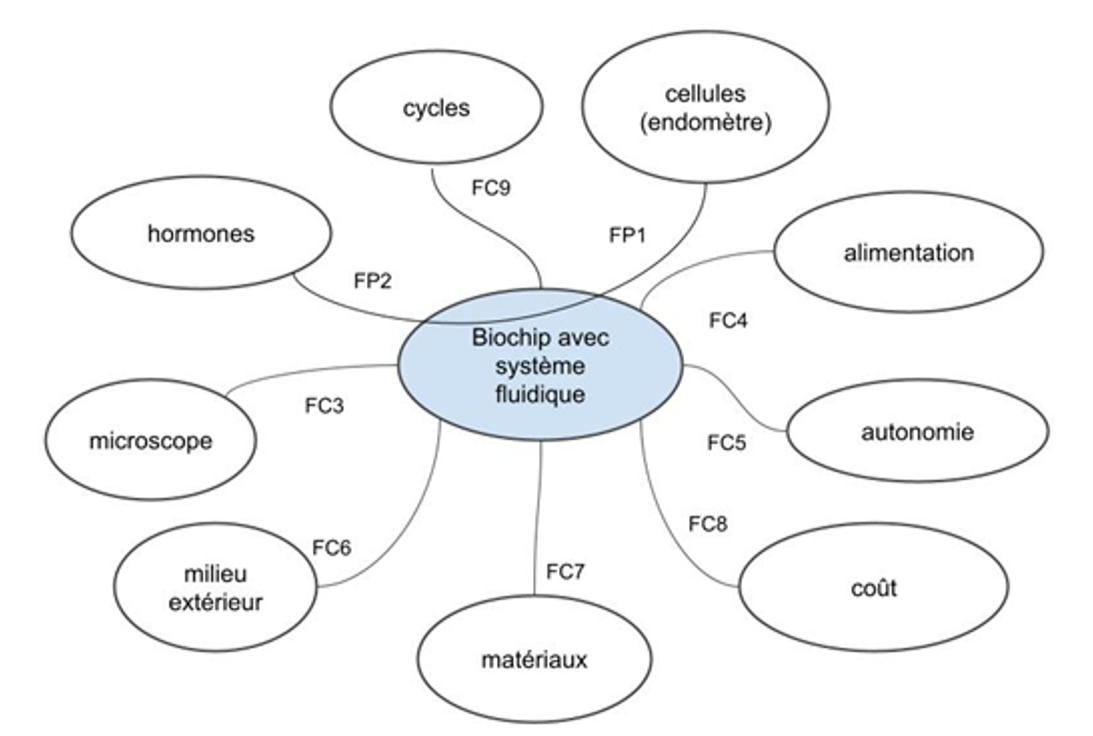
\includegraphics{pieuvre.png}}
    \caption{Diagramme pieuvre avec les fonctions associés}
    \label{fig:pieuvre}
\end{figure}
\subsection{Cahier des charges}
La première fonction à prendre en compte est la survie des cellules.
Pour cela, notre système devra respecter les paramètres suivants :
\begin{itemize}
    \item une température de 37°C
    \item un pH de 7
    \item un renouvellement du milieu de culture de 1 ml par jours
    \item atténué toute variation de milieu
    \item la Biocompatibilité du milieu
\end{itemize}
Pour ce qui est du système fluidique, il permet l'apport du milieu de culture à la cellule et donc nécessite de répondre aux points suivants :
\begin{itemize}
    \item un système étanche
    \item un écoulement laminaire
    \item un système de purge
    \item un système d'injection d'hormones
    \item un mélangeur pour éviter des pics de concentration
    \item une pompe pour un système dynamique
\end{itemize}
Enfin, le système dans sa globalité devra assurer :
\begin{itemize}
    \item une autonomie de 28 jours minimum
    \item une zone transparente permettant l'observation des cellules
\end{itemize}
\subsection{Catalogue de solutions}
\subsubsection{Gestion des nutriments, déchets et de la concentration des hormones}
\begin{table}[H]
    \centering
    \begin{tabular}{|l|l|l|}
        \hline
        \multicolumn{1}{|c|}{\textbf{Solution}}        & \textbf{Avantages}                                                                                                     & \textbf{Inconvénients}                                                                                                             \\ \hline
        Seringues auto-poussés                         & \begin{tabular}[c]{@{}l@{}}-Précis\\ -Facile d'utilisation\\ -Facilement programmable\\ -Réponse linéaire\end{tabular} & \begin{tabular}[c]{@{}l@{}}-Energie\\ -Limité en quantité\\ -Espace\end{tabular}                                                   \\ \hline
        \rowcolor[HTML]{CBCEFB}
        Pompe péristaltiques\cite{pompe_peristaltique} & -Déjà présent au labo                                                                                                  & \begin{tabular}[c]{@{}l@{}}-Peu précis\\ -Energie\end{tabular}                                                                     \\ \hline
        Système de goutte à goutte                     & \begin{tabular}[c]{@{}l@{}}-Low-cost\\ -Economique en énergie\end{tabular}                                             & \begin{tabular}[c]{@{}l@{}}-Précision\\ -A pression atmosphérique\\ -Complexité d'asservissement\\ -Réponse chaotique\end{tabular} \\ \hline
    \end{tabular}
    \caption{Solutions pour la gestions des nutriments, déchets et des hormones}
\end{table}
\subsubsection{Contrôler l'environnement extérieur}
\begin{table}[H]
    \centering
    \begin{tabular}{|l|l|l|}
        \hline
        \multicolumn{1}{|c|}{\textbf{Solution}} & \textbf{Avantages}                                                                                        & \textbf{Inconvénients}                                                                      \\ \hline
        \rowcolor[HTML]{CBCEFB}
        Incubateur                              & \begin{tabular}[c]{@{}l@{}}-Constante externe stable\\ -A disposition\\ -Retour d'expérience\end{tabular} & \begin{tabular}[c]{@{}l@{}}-Placé dans l'incubateur\\ -Protéger l'électronique\end{tabular} \\ \hline
        Système autonome                        & -Pas de dépendance                                                                                        & \begin{tabular}[c]{@{}l@{}}-Compliqué à réaliser\\ -Energivore\\ -Coût\end{tabular}         \\ \hline
    \end{tabular}
    \caption{Solutions pour gérer l'environnement extérieur}
\end{table}
\subsubsection{Cultiver les cellules}
\begin{table}[H]
    \centering
    \begin{tabular}{|l|l|l|}
        \hline
        \multicolumn{1}{|c|}{\textbf{Solution}} & \textbf{Avantages}                                                                                         & \textbf{Inconvénients}                                                             \\ \hline
        \rowcolor[HTML]{CBCEFB}
        Bio-chip en PMMA                        & \begin{tabular}[c]{@{}l@{}}-Usinage\\ -Retour d'expérience\\ -Sur mesure\\ -Fluidique intégré\end{tabular} & \begin{tabular}[c]{@{}l@{}}-Assemblage par couche\\ -Long à fabriquer\end{tabular} \\ \hline
        Boîte de pétris                         & \begin{tabular}[c]{@{}l@{}}-Coût\\ -Stérilité\end{tabular}                                                 & -Pas de circulation de fluide                                                      \\ \hline
    \end{tabular}
    \caption{Solutions pour le milieu de culture}
\end{table}
\subsubsection{Circulation du fluide}
\begin{table}[H]
    \centering
    \begin{tabular}{|l|l|l|}
        \hline
        \multicolumn{1}{|c|}{\textbf{Solution}} & \textbf{Avantages}                                                                                            & \textbf{Inconvénients}                                           \\ \hline
        \rowcolor[HTML]{CBCEFB}
        Pompe péristaltique                     & \begin{tabular}[c]{@{}l@{}}-Déjà présent au labo\\ -Facile d'utilisation\\ -Pas de contamination\end{tabular} & \begin{tabular}[c]{@{}l@{}}-Débit limité\\ -Energie\end{tabular} \\ \hline
        Gravité                                 & \begin{tabular}[c]{@{}l@{}}-Pas besoin de matériel spécifique\\ -Pas besoin d'alimentation\end{tabular}       & -Compliqué à mettre en oeuvre                                    \\ \hline
    \end{tabular}
    \caption{Solutions pour injecter les différents fluides}
\end{table}
\subsubsection{Mélanger les fluides}
\begin{table}[H]
    \centering
    \begin{tabular}{|l|l|l|}
        \hline
        \multicolumn{1}{|c|}{\textbf{Solution}} & \textbf{Avantages}                                                                                                           & \textbf{Inconvénients}                                                                                  \\ \hline
        \rowcolor[HTML]{CBCEFB}
        Mélangeur hydrostatique "2D"            & \begin{tabular}[c]{@{}l@{}}-Economique\\ -Facilité d'intégration\\ -Compact\\ -Volume sur mesure\\ -Modélisable\end{tabular} & \begin{tabular}[c]{@{}l@{}}-A créer\\ -Perte de charge\end{tabular}                                     \\ \hline
        Mélangeur hydrostatique "3D"            & \begin{tabular}[c]{@{}l@{}}-Economique\\ -Facilité d'intégration\\ -Compact\\ -Volume sur mesure\\ -Modélisable\end{tabular} & \begin{tabular}[c]{@{}l@{}}-A créer\\ -Perte de charge\\ -Usinage\end{tabular}                          \\ \hline
        Mélangeur magnétique                    & \begin{tabular}[c]{@{}l@{}}-Déjà présent au labo\\ -Facilement nettoyable\\ -Gestion de la puissance\end{tabular}            & \begin{tabular}[c]{@{}l@{}}-Espace\\ -Biocompatibilité\\ -Non modélisable\\ -Non pilotable\end{tabular} \\ \hline
    \end{tabular}
    \caption{Solutions pour assurer l'homogénéité des liquides}
\end{table}
\subsubsection{Analyser les concentrations}
\begin{table}[H]
    \centering
    \begin{tabular}{|l|l|l|}
        \hline
        \multicolumn{1}{|c|}{\textbf{Solution}} & \textbf{Avantages}                                                                                                                  & \textbf{Inconvénients}                                                                           \\ \hline
        \rowcolor[HTML]{CBCEFB}
        Colorimètre externe                     & \begin{tabular}[c]{@{}l@{}}-Facilité d'intégration\\ -Précis\\ -Déjà présent au labo\end{tabular}                                   & \begin{tabular}[c]{@{}l@{}}-Aucune donnée interne\\ -Nécessite présence utilisateur\end{tabular} \\ \hline
        Colorimètre interne                     & \begin{tabular}[c]{@{}l@{}}-Retour en temps réel\\ -Gain de précision de l'asservissement\\ -Donnée interne au système\end{tabular} & \begin{tabular}[c]{@{}l@{}}-A créer\\ -Précision\end{tabular}                                    \\ \hline
    \end{tabular}
    \caption{Solutions pour contrôler les concentrations}
\end{table}
\subsubsection{Contrôler le système (microcontrôleur)}
\begin{table}[H]
    \centering
    \begin{tabular}{|l|l|l|}
        \hline
        \multicolumn{1}{|c|}{\textbf{Solution}} & \textbf{Avantages}                                                                                                                                      & \textbf{Inconvénients}                                                                                                                           \\ \hline
        Arduino Uno                             & \begin{tabular}[c]{@{}l@{}}-Facilité d'utilisation\\ -Flexible\end{tabular}                                                                             & \begin{tabular}[c]{@{}l@{}}-Pas de stockage interne\\ -Pas de contrôle à distance\\ -Pas de possibilité d'utiliser python\\ -14 pin\end{tabular} \\ \hline
        \rowcolor[HTML]{CBCEFB}
        Raspberry Pi                            & \begin{tabular}[c]{@{}l@{}}-Retour en temps réel\\ -Contrôlable à distance\\ -Stockage interne\\ -Utilisation possible de Python\\ -40 pin\end{tabular} & -Faible disponibilité                                                                                                                            \\ \hline
    \end{tabular}
    \caption{Solutions pour commander le système}
\end{table}
\subsubsection{Alimentation}
\begin{table}[H]
    \centering
    \begin{tabular}{|l|l|l|}
        \hline
        \multicolumn{1}{|c|}{\textbf{Solution}} & \textbf{Avantages} & \textbf{Inconvénients}                                              \\ \hline
        \rowcolor[HTML]{CBCEFB}
        Secteur                                 & -Disponibilité     & -Toujours branché                                                   \\ \hline
        Batteries                               & -Portable          & \begin{tabular}[c]{@{}l@{}}-Prix\\ -Recharge compliqué\end{tabular} \\ \hline
    \end{tabular}
    \caption{Solutions pour alimenter le bio-chip}
\end{table}
\subsection{Schéma bloc du système}
\begin{figure}[H]
    \centering
    \resizebox{\linewidth}{!}{\includegraphics{schema\_block.png}}
    \caption{Schéma bloc du système}
    \label{fig:schema_block}
\end{figure}
\subsection{Déroulé du projet}
insert diagramme de gant
\subsection{Choix pour le projet}
Nous estimons que pour réaliser la culture de cellule de l'endomètre, tout en respectant le cahier des charges, il faut concevoir notre propre bio-chip. Pour ce faire on va utiliser différents outils disponibles dans le laboratoire afin de diminuer les coûts. Certaines pièces devront être fabriqués afin de répondre à nos besoins comme le boitier de notre bio-chip.
Pour accueillir nos cellules nos utiliserons un boitier en PMMA que nous fabriquerons sur place grâce à la découpe laser qui se trouve dans le campus.
Pour la régulation de l'environnement on utilisera un incubateur présent dans le laboratoire car cela diminuera le cout de fabrication.
Nous utiliserons un Raspberry pi pour contrôler notre bio-chip car il dispose de beaucoup plus d'avantage que l'Arduino UNO et il nous permettra de contrôler notre bio-chip à distance.
Pour l'apport d'hormones et de nutriment on utilisera des pousses seringues qui sont disponible dans le laboratoire.
Pour faire circuler le fluide dans notre boitier on prendra des pompes péristaltiques qui sont fournis.
L'ensemble du bio-chip sera alimenté par le secteur afin de limiter les coûts de fabrication et éviter de devoir développer un système avec une batterie

\newpage
\section{Conception mécanique}
\subsection{Mélangeur hydrostatique}
\subsubsection{Simulation fluidique}
\subsubsection{CAO du mélangeur}
\subsection{Zone de culture}
\subsection{Support des réservoirs}

\newpage
\section{Conception électronique et programmation}
\subsection{Carte d'alimentation}
L'alimentation de tous le biochip se fera via l'alimentation d'un Arduino de 60 W.
Il arrive sur la carte d'alimentation via la connectique circulaire JAlim.
U1 est un régulateur de tension à découpage de la marque TRACO, il permet de descendre la tension de 12V à 5V il sert à alimenter le Raspberry pi qui sera alimenter par ses pins GPIO.
Les moteurs seront contrôlés par les mosfet M1, M2 et M3.
Les moteurs seront branchés à la carte via des connecteurs circulaire afin que le système soit le plus flexible possible.
Les diodes D1, D2 et D3 sont des diodes de roues libres.
\subsection{Programmation}
\subsubsection{GitHub}
On a mis en place un GitHub pour se partager les codes de programmation, le "repo" contient aussi une ébauche du guide d'utilisateur.
Le guide d'utilisateur contient actuellement uniquement les requirements pour le Raspberry pi ainsi que les commandes à utiliser.
\subsubsection{Raspberry Pi}
On a configuré le Raspberry pi 4 pour qu'on puisse se connecter dessus à distance à l'aide du protocole SSH.
On peut s'y connecter facilement dessus à partir du moment que l'on se trouve sur le même réseau wifi.
On peut lui transmettre des fichiers ainsi que récupérer des fichiers qui sont stockées dessus.
\subsubsection{Préparation des données}
Ce code permet de préparer les datas afin de pouvoir être utiliser par le logiciel qui contrôle le biochip.
Il a été conçu pour que l'utilisateur rentre un minimum de donner afin de gagner du temps.
Il permet de convertir un fichier csv que l'utilisateur aura créée au préalable avec les différents jalons de concentration en un fichier qui contient toutes les concentrations de l'expérience sur 28 jours.
Sur la figure \ref{fig:dataPreparation} on peut voir une représentation des données rentrées par l'utilisateur et les données produites par le programme.
\begin{figure}[H]
    \centering
    \resizebox{\linewidth}{!}{\includegraphics{representation\_data\_gen.png}}
    \caption{Données généré par le programme avec les données rentrées par l'utilisateur}
    \label{fig:dataPreparation}
\end{figure}
On peut l'utiliser directement sur un ordinateur puis envoyer le fichier généré sur le Raspberry pi ou bien on peut envoyer le fichier csv sur le Raspberry pi puis le généré directement sur le Raspberry pi.
Le fichier généré est un fichier de type ftr il n'est donc pas lisible directement ceci est fait afin de gagner en rapidité d'exécution et gagner du stockage.
Si on utilisait un fichier csv équivalent il contiendrait tellement de donnés qu'il faudrait plusieurs secondes pour le généré et il prendrait 10 fois plus de stockage.
Le fichier à préparer doit être présenter sous la forme :
\begin{table}[H]
    \centering
    \begin{tabular}{lll}
        Time & Conc1 & Conc2 \\
        0    & 1     & 1     \\
        2    & 6     & 8     \\
        10   & 2     & 1     \\
        15   & 4     & 2
    \end{tabular}
\end{table}
\newpage
\section{Conclusion}

\newpage
\section{Annexe}

\newpage
\printbibliography

\end{document}